\section{System Architecture}

The FlashBoost architecture is composed of multiple identical nodes. Each node
consists of a host server and a FlashBoost storage device. The host servers are
networked together using Ethernet or other general-purpose networking fabric.
The FlashBoost storage device consists of a in-store processing engine, flash
storage and flash controller, host interface, and a high-speed network controller.
The in-store processing engine can implement a raw
access to flash and network resources, an application-specific hardware
accelerator, or both. The host software can send high-level requests over the
PCIe link to the in-storage processing engine to access flash network and computation resources.
In our implementation of FlashBoost, we have used a Field Programmable Gate
Array (FPGA) to implement The in-store processor and also the flash, host and
network controllers. However, the FlashBoost Architecture should not be limited
to an FPGA-based implementation.


\begin{figure*}[ht]
	\begin{center}
	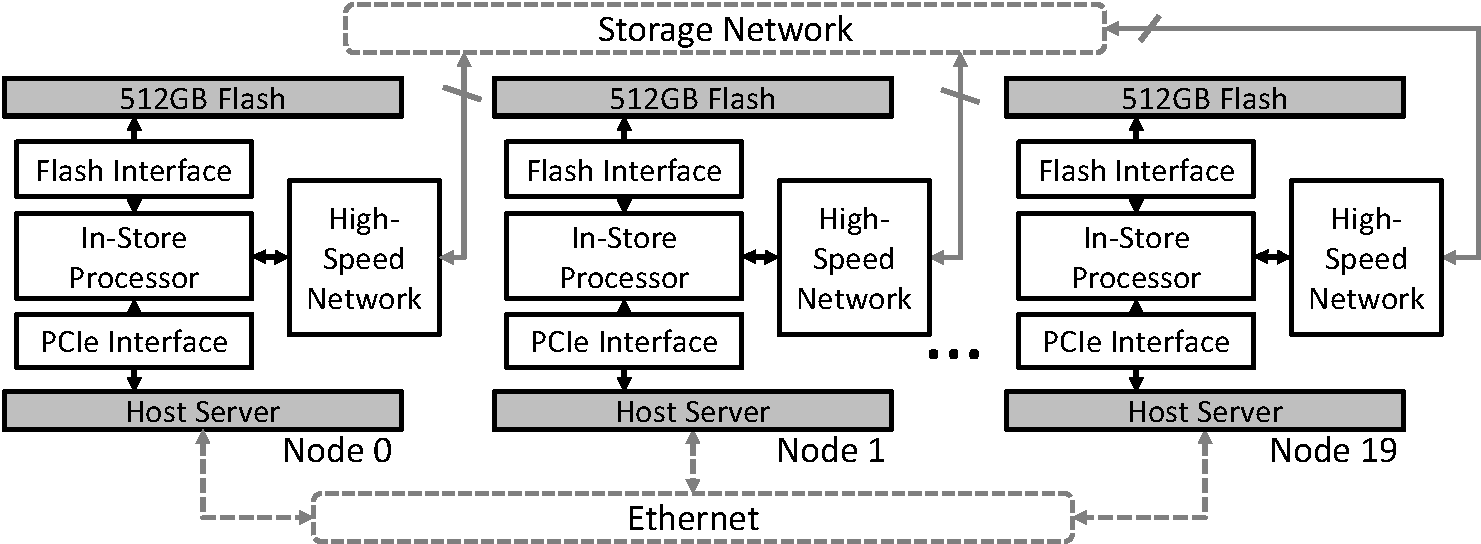
\includegraphics[width=0.8\paperwidth]{figures/architecture.pdf}
	\caption{FlashBoost Architecture}
	\label{fig:architecture}
	\end{center}
\end{figure*}


The in-store processing engine has access to four major services, The flash
controller, network controller, host interface and the DRAM Buffer.
Figure~\ref{fig:ispservice} shows the four services. Development of FlashBoost was
done in the high-level hardware description language Bluespec. As a result, all
services expose a high-level language interface using latency-insensitive FIFOs
for communication. This makes the services intuitive to use, and flexible to be
used easily with many in-storage processing engines.

\begin{figure}[h]
	\begin{center}
	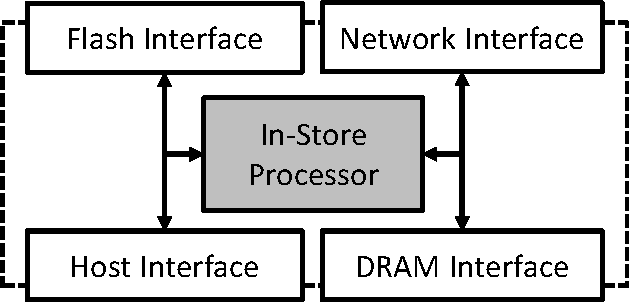
\includegraphics[width=0.3\paperwidth]{figures/isp-service-crop.pdf}
	\caption{Services Provided to In-Store Processor}
	\label{fig:ispcore}
	\end{center}
\end{figure}

\subsection{Flash Interface}

Access to flash storage is provided by the flash controller via a
fast, low-level and error-free interface with minimal bandwidth and
latency overhead. This interface exposes the internal memory organization of
the flash device, namely the buses/channels, chips, blocks and pages.
The interface is designed to stream data in
and out of the flash chips as fast as possible without concern for
flash management. Garbage collection, bad block management and
wear-leveling functionalities are handled by the flash-aware file system
in the host kernel (discussed in Section~\ref{?}). The key advantage of such
a low-level interface is that in-store processors have direct access to
the data in a streaming fashion with minimal buffering and insignificant
latency overhead. 

The raw flash interface, in hardware, is defined below:

%[captionpos=b, caption={Flash Controller Interface}, label={lst:hwifc}]
\begin{lstlisting}
interface FlashIfc;       
  method sendCmd (FlashOp op, Bit#(4) bus,
                  Bit#(3) chip, Bit#(16) block, 
                  Bit#(8) page, Bit#(8) tag);        
  method writeWord (Bit#(128) data, Bit#(8) tag);
  method Tuple2#(Bit#(128), Bit#(8)) readWord (); 
  method Bit#(8) writeDataReq ();
  method Tuple2#(Bit#(8), StatusT) ackStatus ();
endinterface 
\end{lstlisting}

To access the flash, the user issues a flash command
(\textit{sendCmd} method) with the operation, the address and
a free tag. For writes, the user awaits for a write data request from
the controller scheduler (\textit{writeDataReq} method), and then sends
the write data corresponding to that request in 128-bit bursts
(\textit{writeWord} method). An acknowledgement is received when the
operation completes (\textit{ackStatus} method). For read operations,
data will return in 128-bit bursts along with the command tag that the
burst corresponds to. We emphasize that for maximum performance, the
controller sends these data bursts \textbf{out of order} with respect to
the issued request and \textbf{interleaved} with other read requests.
Thus completion buffers may be required on the user side. Furthermore,
we note that to saturate the bandwidth of the flash device, multiple
commands must be in-flight at the same time, since flash operations
have latencies of tens to thousands of microseconds. 

In our architecture, multiple users may need shared access to the
flash controller interface. For example, a particular flash controller may
be accessed by local in-store processors, local host software over PCIe
DMA, or remote in-store processors. Thus, we include as part of the
platform, an interface multiplexer that converts one flash interface
into a parametrizable number of additional interfaces. 

%TODO: give a name to this module?
To ease development of hardware accelerators (i.e. in-store processors),
we also provide a parametrizable module that converts a flash interface
into multiple simple in-order request/response interfaces
(Figure~\ref{?}). We allow the user to adjust the interface width, the
command queue depth and number of interfaces of the converter.
Internally, the converter renames tags and uses completion buffers to
order data. This design easily permits multiple accelerators to be
attached to the flash device, taking advantage of flash parallelism. 


\begin{figure}[h]
	\begin{center}
	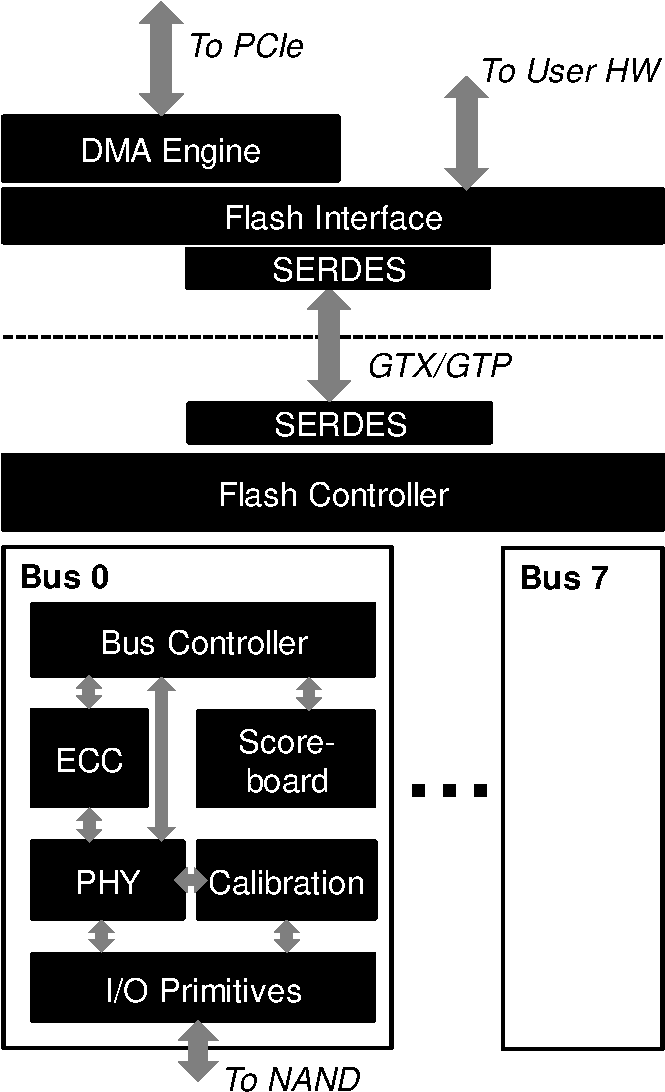
\includegraphics[scale=0.4]{figures/top-arch-crop.pdf}
	\caption{Flash Interface}
	\label{fig:flashinterface}
	\end{center}
\end{figure}

\subsection{Inter-Storage Network}

Conventional general-purpose networking infrastructures such as TCP are designed to serve
all kinds of network traffic over any distance, ranging from intra-rack to over
continents. This makes the protocol incredibly complex and results in a large
protocol overhead.

The near-data processors in FlashBoost are linked together using a separate
high-performance network among themselves in which all nodes have multiple
network ports and act both as a network switch as well as an endpoint. This network provides low-level
routing, some flow control and use of virtual channels, but omits various high level
features that modern network protocols provide. From the in-storage processing
engine's point of view, the network looks like a variable number of FIFOs, all
of which can be declared to be of different bit-width according to the use. The
network FIFOs have features that are expected of normal FIFOs, such as back
pressure. The network FIFOs also act as virtual link endpoints. Such intuitive characteristics of the network should aid in the ease
of in-storage processor development. The use of the network looks like the following, in pseudocode:

\begin{verbatim}
NetworkEndpoint#(type Bit#(64)) endpoint1 
     <- mkNetworkEndpoint(1); // endpoint id: 1
NetworkEndpoint#(type Bit#(32)) endpoint2 
     <- mkNetworkEndpoint(8); // endpoint id: 8
List endpoints = 
     cons(endpoint1, cons(endpoint2, nil));
NetworkArbiter arbiter 
     <- mkNetworkArbiter(endpoints);

...
endpoint1.send(data,dest);

...
tuple(data,src) <- endpoint1.receive;
\end{verbatim}

In our FlashBoost implementation, this network is implemented using the
low-latency serial links that are already included in the FPGA. By implementing
routing in the hardware and using a very low-latency network fabric, we were
able to achieve very high performance, with 0.5$\mu s$ of latency per network
hop, and near 10Gbps of bandwidth per link. Our implementation has a network
fan-out of 8 ports per storage node, so the aggregate network bandwidth
available to a node is up to 10Gbps.

\subsubsection{Link Layer}

The link layer managed physical connections between network ports in the storage
nodes. The most important aspect of the link layer is the simple token-based
flow control implementation. This assures that no packet will drop if the data
rate is higher than what the network can manage, or if the data is not received
from the destination node quick enough.

\subsubsection{Routing Layer}

Figure~\ref{fig:networkinterface} shows the implementation of the router in each
storage node. Each packet can either come from the network port's link layer
interface, or from the user's network endpoint. Each incoming packet's
destination field is compared to the routing table in the router to determine
whether to be forwarded to a remote node via a network port, or to be delivered
to a local endpoint if its destination is the current node. It then goes through
one of the four crossbar switches to be delivered to the correct destination. 
Fairness is implemented using a round-robin priority ordering to ensure maximum
throughput while ensuring no port starves.

It is important to note that the routing table can have more than one network
port entry per destination node index. This is because each pair of nodes can
have more than one immediate link connecting between them, and there may be
multiple viable paths between a pair of two remote nodes. In order to make
maximum use of the available bandwidth in such cases, the routing table can have
entries for multiple valid ports for the next hop. In order to ensure in-order
arrival, the endpoint id of the origin endpoint is hashed to deterministically
decide which entry to use in the routing table. In-order arrival is desirable in
a hardware implementation because completion buffers may be expensive.
Because of this characteristic, if the in-storage processing engine want to
ensure more bandwidth, it can break a wide data bus into multiple endpoints and
send data over them in parallel. Figure~\ref{fig:networkrouting} shows packet
routing in an example network.

\begin{figure}[h]
	\begin{center}
	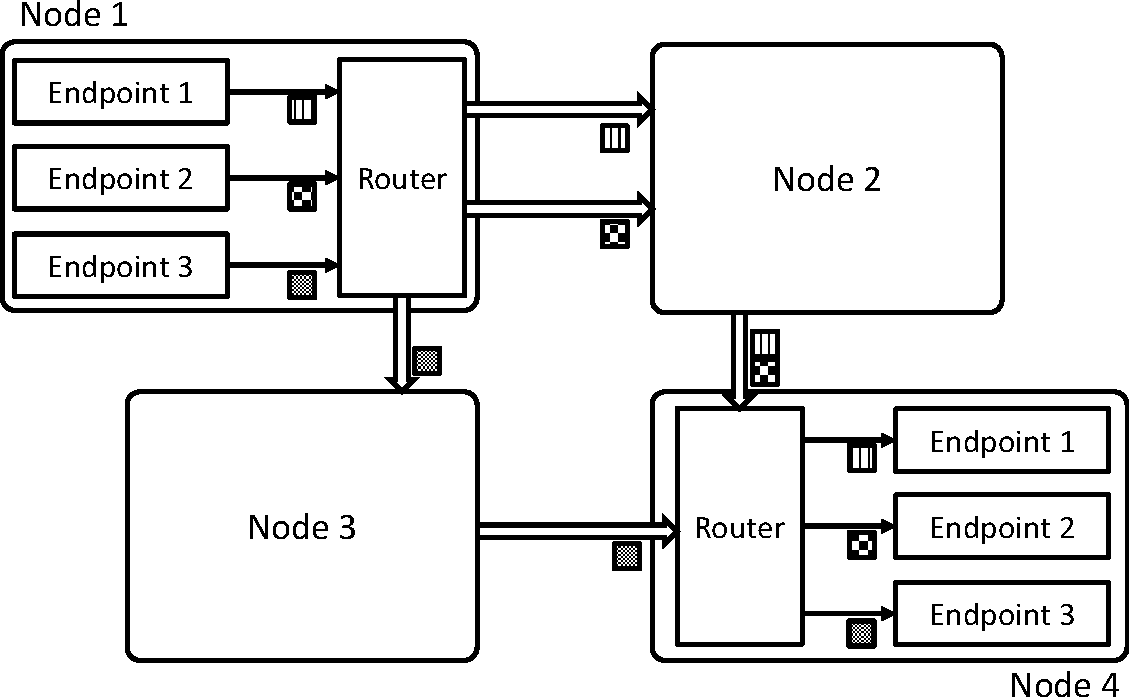
\includegraphics[width=0.4\textwidth]{figures/routing-crop.pdf}
	\caption{Routing Packets Across the Network}
	\label{fig:networkrouting}
	\end{center}
\end{figure}

It should be pointed out that because end-to-end flow control doesn't exist, a
large part of the network might actually block if a destination endpoint doesn't
receive the data quick enough. This was an intentional design choice to build an
extremely low-latency network while maintaining low resource usage. If the designer is sure that the packets will
always be consumed, end-to-end flow control can be omitted. Otherwise, the
designer can choose to implement a flow control protocol using the network
endpoints. We plan to provide pre-implemented flow control modules that can be
plugged in.

\begin{figure}[h]
	\begin{center}
	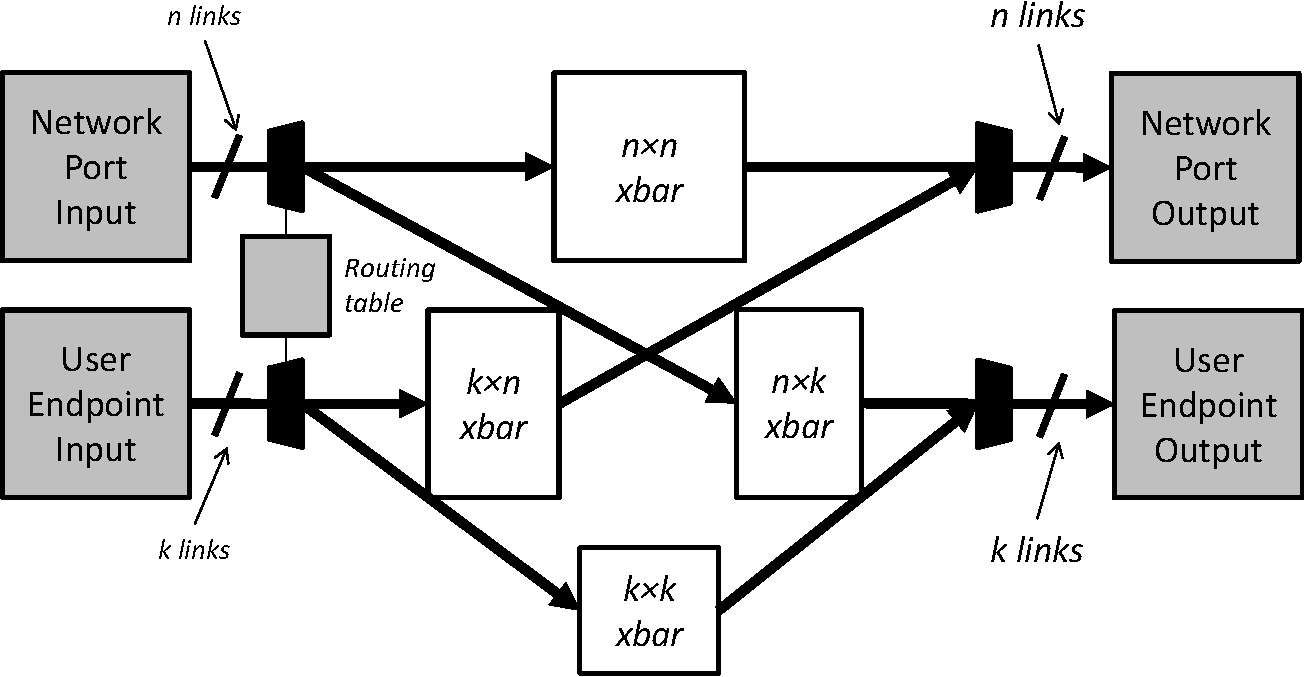
\includegraphics[scale=0.4]{figures/network-routing-crop.pdf}
	\caption{Network Interface}
	\label{fig:networkinterface}
	\end{center}
\end{figure}


\subsection{Host Interface}

The near-data processing core can be accessed from the host server over either a
low-level RPC-like interface or a file system abstraction. Our host interface
was implemented using Connectal~\ref{connectal}, a hardware-software codesign
framework built by Quanta Research Cambridge. Connectal reads the interface
definition file written by the programmer and generates glue logic between
hardware and software. Connectal provides an RPC-like interface, as well as a
memory-mapped DMA interface for high bandwidth data transfer.

The software maintains two 128-page page buffers, each for reads and writes. When
issuing a read or write request, the software sends the target or source page
buffer index along with the request to let the hardware side host interface know
where to read or write data from. Since this buffer is returned to the free list
when each operation is finished the buffer index effectively acts as the locally
unique tag for each flash operation. Writing data is straightforward, as data is
read in-order from the host page buffer and written in-order to each flash
controller bus. However, reading from flash is slightly more complex because the
data from each flash chip can come interleaved, even within the same bus. 
We include an implementation of a multiple-in-single-out completion buffer using
on-chip BRAM with burst support, in order to save hardware resources by not
having 128 separate FIFOs.

Reading or writing data from the host buffers were done by DMA read/write
engines implemented in the Connectal framework. In our FlashBoost
implementation, there are four read engines and four write engines each, in
order to more easily make maximum use of the PCIe bandwidth. Since there are 16
busses in total per storage node, each read/write engines manage data from four
busses each.
Figure~\ref{fig:hostinterface} describes the
structure of the host interface.

\begin{figure}[ht!]
	\centering
%	\subfloat[Writing Data to Storage]
%		{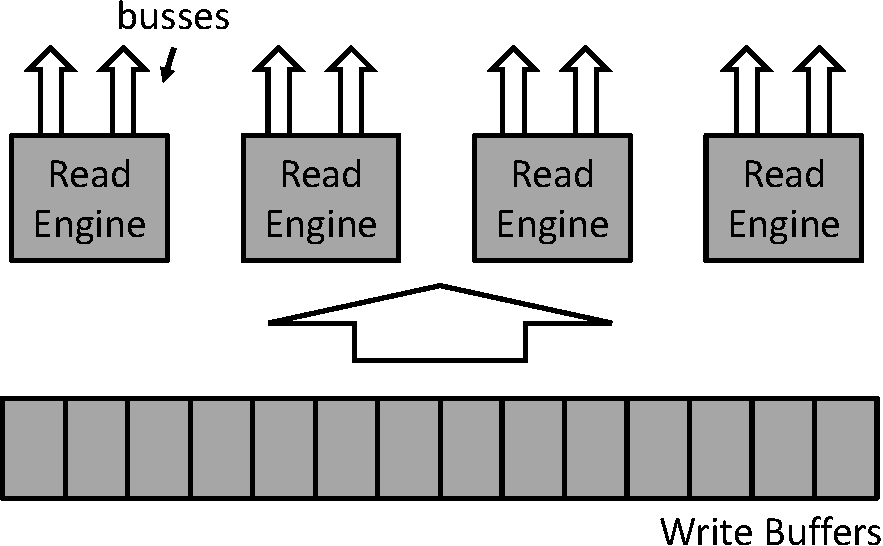
\includegraphics[width=0.23\textwidth]{figures/readinterface-crop.pdf}}
%	\subfloat[Reading Data from Storage]
%		{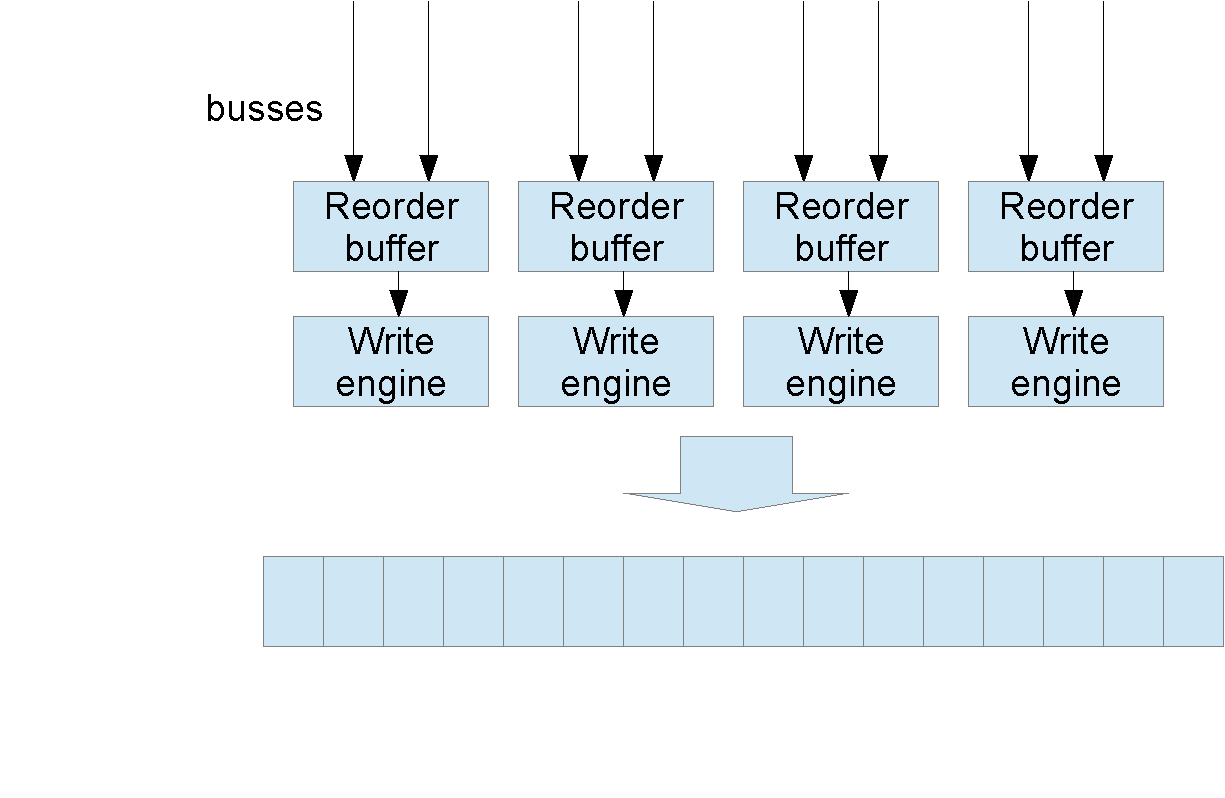
\includegraphics[width=0.23\textwidth]{figures/writeinterface-crop.pdf}}
	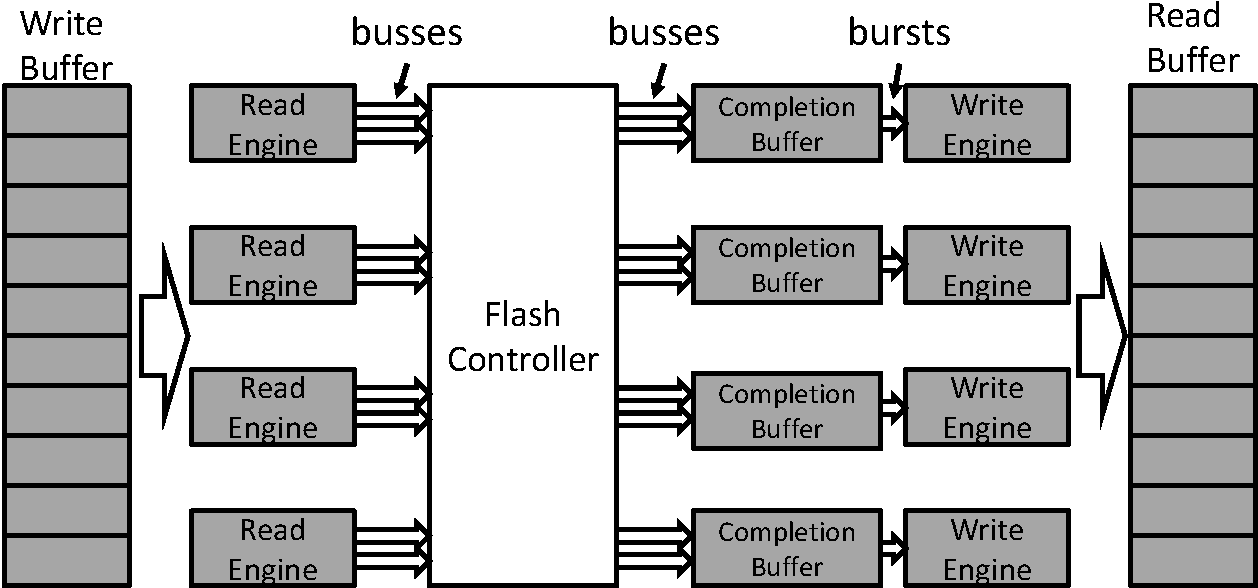
\includegraphics[width=0.4	\textwidth]{figures/hostinterface-crop.pdf}
	\caption{Host-FPGA Interface Over PCIe}
	\label{fig:hostinterface}
\end{figure}

%TODO: \subsubsection{Storage Bridge to Host}

\subsection{File System Interface}

NAND flash has very different characteristics from traditional hard disk drives,
so it is required to run a flash-aware management layer like a flash translation
layer (FTL)~\cite{}.  We develop a refactored I/O architecture that offloads
almost all of the FTL functions into a log-structured file system, called
RFS~\cite{}. Unlike the conventional FTL design, RFS performs logical-to-
physical mapping and garbage collection, achieving better garbage collection
efficiency at much lower memory requirement. For the sake of compatibility with
existing software, FlashBoost also offers a full-fledged page-level FTL for
end-users, which is implemented in the device driver like Fusion IO’s driver. It
allows us to use well-known Linux file systems (e.g., ext2/4/3) as well as
database systems (directly running on top of a block device) with FlashBoost.

The most important feature of the FlashBoost software is that it provides
easy-to-use interfaces for application-specific hardware accelerators, allowing
end-users to easily make use of fast near-data processing without any efforts to
write their own custom interfaces manually. By leveraging the HW/SW interfaces
generation of Connectal~\cite{}, FlashBoost automatically creates SW proxies
(i.e., C functions and C++ classes) and HW wrappers according to the HW/SW
specifications of end-users. In FlashBoost, user-level applications send
application- specific queries to the storage device using SW proxies, together
with physical locations of data in NAND flash to analyze using hardware
accelerators. Those physical locations can be easily obtained from the file
system (i.e., RFS) or the device driver because they maintain mapping
information between user files and NAND flash. After near-data processing is
done, hardware accelerators inform user applications of analysis results via HW
wrappers. Thus, a large amount of data transfer between the host and the storage
device can be avoided. User queries are sent to the hardware directly, bypassing
the OS kernel, except for essential driver modules. This helps us to avoid deep
kernel stacks that often cause long I/O latencies. It is common that multiple
user-applications compete for the limited and precious hardware acceleration
units. For efficient sharing of hardware resources, FlashBoost runs a scheduling
daemon that assigns available hardware-acceleration units to competing
user-applications. In our implementation, a simple FIFO-based policy is used for
request scheduling.

\begin{figure}[h]
	\begin{center}
	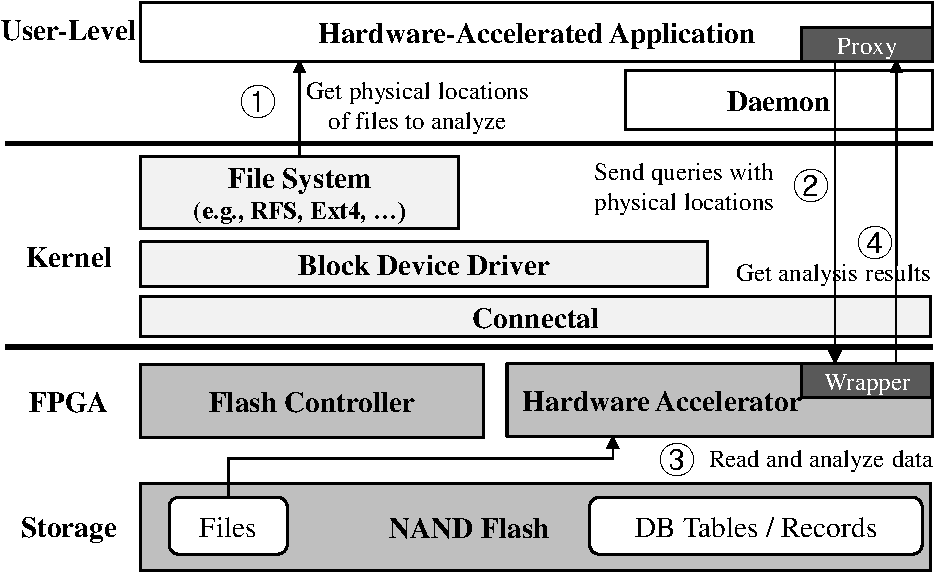
\includegraphics[width=0.4\paperwidth]{figures/software.pdf}
	\caption{File System Interface}
	\label{fig:filesystem}
	\end{center}
\end{figure}
